% - template colors
\documentclass{beamer}

% SETUP
\usepackage{morris}
\definecolor{purple}{rgb}	{0.69, 0.38, 0.53}
\definecolor{orange}{rgb}	{0.84, 0.36, 0.05}
\definecolor{blue}{rgb}	{0.27, 0.52, 0.53}
\definecolor{green}{rgb}	{0.6, 0.59, 0.1}
\definecolor{red}{rgb}	{0.8, 0.14, 0.11}
\definecolor{yellow}{rgb}	{0.84, 0.6, 0.13}
\definecolor{aqua}{rgb}	{0.41, 0.62, 0.42}
\definecolor{extlinkcolor}{rgb}	{0.03, 0.4, 0.47}
\definecolor{intlinkcolor}{rgb}	{0.69, 0.23, 0.01}

\DeclareMathOperator{\elbo}{ELBO}
\DeclareMathOperator*{\erf}{erf}

\newcommand{\aprxpost}{{q_{\B{\φ}_k}(\s_k|\m)}}

% Following are some really short macros!
\newcommand\D{\ensuremath{\mathcal{D}}}
\newcommand\m{\ensuremath{\B{m}}}
\newcommand\s{\ensuremath{\B{s}}}
\newcommand\z{\ensuremath{\B{z}}}
\newcommand\x{\ensuremath{\B{x}}}

\newcommand{\decrvalue}[2]{\the\numexpr\value{#1}-#2\relax}


\definecolor{primary}{HTML}{524667}

\usetheme[numbering=fraction,block=fill]{metropolis}
\setbeamercolor{normal text}{fg=black, bg=white}

\setbeamercolor{palette primary}{%
    fg=white,
    bg=primary
}

\graphicspath{{graphics/}} % set of paths to search for images

\usepackage{tikz}
\usepackage{tikz-bayesnet}
\usetikzlibrary{
    3d,
    arrows,
    arrows.meta,
    backgrounds,
    bending,
    calc,
    chains,
    decorations.pathmorphing,
    decorations.pathreplacing,
    graphs,
    matrix,
    patterns,
    positioning,
    quotes,
    shapes.arrows,
    shapes.geometric,
    shapes.misc,
}
\tikzset{>=latex}
\tikzset{every picture/.style={/utils/exec={\sffamily}}}

\usepackage{pgfplots}
\usepgfplotslibrary{
    groupplots,
    dateplot,
}
\pgfplotsset{compat=newest}
\usepackage[size=footnotesize]{subcaption}
\usepackage[font=footnotesize]{caption}

\usefonttheme{serif}
\usefonttheme{professionalfonts}
\usepackage{mathpazo}
\usepackage{euler}
\setbeamerfont{footnote}{size=\tiny}

% ----------------------------------------------------------------------------------------------------------------------------------------

% META DATA
\title{Unsupervised musical source separation}
\date{\today}
\author{Maurice Frank}
\institute{\textsc{amsterdam machine learning lab\\university of amsterdam}}

\begin{document}
    \maketitle

    \begin{frame}{The problem setup}
        \begin{figure}
            \centering
            \begin{tikzpicture}
    \node[draw] (mix) {Mix\quad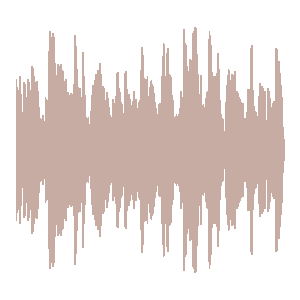
\includegraphics[width=30pt]{wave/mix.pdf}};
    \draw[arrows=-{Triangle[open, angle=60:3mm]}] ([xshift=-17pt]mix.west) -- (mix.west);
    \draw (mix.east) -- ([xshift=17pt]mix.east);

    \foreach \source/\offset in {other/0,drums/1,vocals/2,bass/3}{%
        \node[above left=-2.2+\offset and 25pt of mix.west] (wave_\source) {\includegraphics[width=30pt]{wave/\source.pdf}};
        \node[left=0 of wave_\source] (img_\source) {\includegraphics[width=30pt]{../data/images/\source.png}};
        \draw (wave_\source) -| ([xshift=-17pt]mix.west);
        \node[above right=-1.6+\offset and 30pt of mix.east] (output_\source) {};
        \draw[arrows=-{Triangle[open, angle=30:2mm]}] ([xshift=17pt]mix.east) |- (output_\source.west);
    }%

    \node[right=50pt of mix.east] (he) {\Large Undo?};
\end{tikzpicture}

        \end{figure}

        Difference to the \I{cocktail party problem}:\\Sources are different instruments with indivdual characteristics
    \end{frame}

    \begin{frame}{The problem setup: notation}
        Source signals
         \[\B{S} = {[\s_1,\…,\s_N]}^T \∈ \ℝ^{N\× T} \]
        give the mix through the linear mixing function \(f(\·)\)
        \[ \m = f(\B{S}) = \Σ_k^N a_k \s_k \∈ \ℝ^{1\× T}\]
        for which we search for an inverse \(g(\·)\)
        \[g: \ℝ^{1\× T} \to \ℝ^{N\× T}\]
        \[g(\m) \approxeq \B{S}\]
    \end{frame}

    \begin{frame}{The common solution}
        \begin{figure}
            \centering
            \begin{tikzpicture}
    \node[draw] (mix) {Mix\quad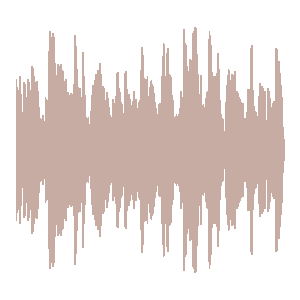
\includegraphics[width=30pt]{wave/mix.pdf}};

    \node[fill=primary, right=30pt of mix.east, inner sep=5pt, text width=70pt] (ann) {{\color{white}some neural network}};
    \draw (ann.east) -- ([xshift=17pt]ann.east);
    \draw (mix.east) -- (ann.west);

    \node[right=50pt of ann.east, align=left] (regr) {regress \\ latent sources};

    \foreach \source/\offset in {other/0,drums/1,vocals/2,bass/3}{%
        \node[above right=-1.6+\offset and 30pt of ann.east] (output_\source) {};
        \draw[arrows=-{Triangle[open, angle=30:2mm]}] ([xshift=17pt]ann.east) |- (output_\source.west);
    }%
\end{tikzpicture}

        \end{figure}

        \begin{itemize}
            \item[]{\makebox[2.2cm]{Optimize:\hfill} \(\argmax_{\B{\θ}} p_{\B{\θ}}(\s_1,\…,\s_N | \m)\)}
            \item[]{\makebox[2.2cm]{Problem:\hfill} Need expensive tuples \((\m,\{\s_1,\…,\s_N\})\)}
        \end{itemize}
    \end{frame}

    \begin{frame}{Bayesian perspective: Graphical model}
        \begin{columns}
            \begin{column}{0.5\textwidth}
                \begin{enumerate}
                    \item Do not learn separation \(\Rightarrow\) Learn generation \(p(\m)\) instead
                    \item Source channels are latent variables and independent
                    \item Extract most likely set of latent values for a given mix \(\B{m}\)
                \end{enumerate}
            \end{column}
            \begin{column}{0.5\textwidth}
                \begin{figure}
                    \centering
                    \begin{tikzpicture}
    \node[obs]                (m) {\(\B{m}\)};
    \node[latent, above=of m]  (s1) {\(\B{s}_1\)};
    \node[latent, above left=of m]  (s2) {\(\B{s}_2\)};
    \node[latent, below left=of m]  (s3) {\(\B{s}_3\)};
    \node[latent, below=of m]  (s4) {\(\B{s}_4\)};

    \edge {s1} {m} ; %
    \edge {s2} {m} ; %
    \edge {s3} {m} ; %
    \edge {s4} {m} ; %

    \plate {ms} {(m)(s1)(s2)(s3)(s4)} {\(N\)} ;
\end{tikzpicture}

                \end{figure}
            \end{column}
        \end{columns}
    \end{frame}

    \begin{frame}{Bayesian perspective: Graphical model}
        \begin{columns}
            \begin{column}{0.5\textwidth}
                Implied assumption
                \[
                    p(\m,\s_1,\…,\s_N) \equiv p(\m|\s_1,\…,\s_N) \· \Π_k^N p(\s_k)
                \]
                that we can model the sources independently (\I{wrong!}).\\

                How to retrieve get sources from the posterior?
                \[
                    \s_1,\…,\s_N \sim p(\s_1,\…,\s_N | \m)
                \]
            \end{column}
            \begin{column}{0.5\textwidth}
                \begin{figure}
                    \centering
                    \begin{tikzpicture}
    \node[obs]                (m) {\(\B{m}\)};
    \node[latent, above=of m]  (s1) {\(\B{s}_1\)};
    \node[latent, above left=of m]  (s2) {\(\B{s}_2\)};
    \node[latent, below left=of m]  (s3) {\(\B{s}_3\)};
    \node[latent, below=of m]  (s4) {\(\B{s}_4\)};

    \edge {s1} {m} ; %
    \edge {s2} {m} ; %
    \edge {s3} {m} ; %
    \edge {s4} {m} ; %

    \plate {ms} {(m)(s1)(s2)(s3)(s4)} {\(N\)} ;
\end{tikzpicture}

                \end{figure}
            \end{column}
        \end{columns}
    \end{frame}

    \begin{frame}{How to get sources from the posterior}
        With prior models \(\{p_k(\s_k)\}_N\) how to get samples from the posterior
        \[
            \s_1,\…,\s_N \sim p(\s_1,\…,\s_N | \m)
        \]
        \begin{itemize}
            \item Sample from the posterior \(\Rightarrow\) SGLD
            \item Model the posterior distribution \(\Rightarrow\) VAE
        \end{itemize}
    \end{frame}

    \begin{frame}{Sampling from the posterior: SGLD}
        With \I{Stochastic Gradient Langevin Dynamics} we can directly sample from the posterior without modeling it.

        Iteratively improve samples \(\s_k\) with gradient update of the prior model and the mixing constraint.
        \[
            \s_k^{(t+1)} = \s_k^{(t)} + \η \· \∇_{\s_k} \left( \log p_k(\s_k^{(t)}) + \÷{1}{2} {\| \m - \Σ_k^N\s_k^{(t)} \|}^2 \right) + 2\·\sqrt{\η}\ε_t
        \]
        Gaussian noise \(\ε\) scaled by the step size \(\η\) is added to avoid local maxima.

        \I{Jayaram \& Thickstun, 2020} proved SGLD for separation for (small) images.
    \end{frame}

    \begin{frame}{Modeling the posterior: VAE}
        Propose an approximate posterior \(\aprxpost\) and we can derive the ELBO:\@

        \begin{align*}
            \E_\aprxpost^N \left[ \log p(\m) \right]
            &= \E_\aprxpost^N \left[ \log \÷{p(\m,\s_1,\…,\s_N)}{p(\s_1,\…,\s_N|\m)} \right]\\
            &\geq \Σ_k^N \E_\aprxpost \left[ \log \÷{p(\s_k)}{\aprxpost} \right]\\
            &\hspace{1em}+\E_\aprxpost \left[ p(\m|\s_1,\…,\s_N) \right]
        \end{align*}
    \end{frame}

    \begin{frame}{Modeling the posterior: VAE}
        Training of the encoders \(\texttt{Encoder}_{\φ_k}: \m \to \μ,\σ\) is done with KL-divergence and MSE loss.
        \[
            \mathcal{L} (\B{\φ}, \m) = \Σ_k^N \KL{[\aprxpost\|p_k(\s_k)]} + {\left( \÷{1}{N} \Σ_k^N a_k\hat{\s}_k - \m \right)}^2
        \]
        \[\hat{\s}_k \sim \aprxpost\]
    \end{frame}

    \section{From theory to practice}

    \begin{frame}{Datasets}
        \begin{columns}
            \begin{column}[T]{0.5\textwidth}
                \texttt{musdb18}
                \resizebox{0.8\textwidth}{!}{%
                    \begin{tikzpicture}
    \node[matrix,thick,column sep=1em,row sep=1em]
    {
        \node (bass)    {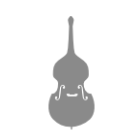
\includegraphics[width=35pt]{../data/images/bass.png}}; &
        \node (drums){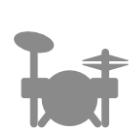
\includegraphics[width=35pt]{../data/images/drums.png}}; &
        \node (voice)  {
\includegraphics[width=35pt]{../data/images/vocals.png}}; &
        \node (other)  {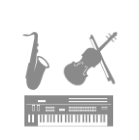
\includegraphics[width=35pt]{../data/images/other.png}}; \\
    };
\end{tikzpicture}

                }%
                \begin{itemize}
                    \item 100 full real songs
                    \item{\small[bass, drums, voice, \I{other}]}
                    \item \I{No} post-mixing effects
                \end{itemize}
            \end{column}
            \begin{column}[T]{0.5\textwidth}
                ToyData
                \resizebox{0.8\textwidth}{!}{%
                    \begin{tikzpicture}
    \node[matrix,thick,column sep=1em,row sep=1em]
    {
        \draw (0,0.5) sin (0.25,1) cos (0.5,0.5) sin (0.75,0) cos (1,0.5); &
        \draw (0,0) -- (1,1) -- (1,0); &
        \draw (0,0) -- (0,1) -- (0.5,1) -- (0.5,0) -- (1,0); &
        \draw (0,0) -- (0.5,1) -- (1,0); \\
    };
\end{tikzpicture}

                }%
                \begin{itemize}
                    \item Simple synthesizer waves
                    \item{\small[sine, saw, sqaure, triangle]}
                    \item Random phase, period and amplitude
                \end{itemize}
            \end{column}
        \end{columns}

        \begin{center}
            Processing:
            \begin{itemize}
                \item Fixed-length frames, around 1sec
                \item Mix is simple mean
            \end{itemize}
        \end{center}
    \end{frame}

    \begin{frame}{Modeling the priors}
        \begin{columns}
            \begin{column}{0.6\textwidth}
                \begin{itemize}
                    \item Model \(\log p_k(\s_k)\) with flow model.
                    \item \(N\) Source priors are trained independently.
                    \item Follow recent FloWaveNet\footnotemark: Coupling layers are parameterized by WaveNets. Large receptive field through squeezing and dilated convolutions.
                \end{itemize}
            \end{column}
            \begin{column}{0.4\textwidth}
                \tikzstyle{box} = [draw, rectangle, inner sep=4mm]
\tikzstyle{arr} = [->, >={triangle 45}]
\tikzstyle{var} = [circle,fill=white,draw=black,inner sep=1pt, minimum size=20pt]

\begin{tikzpicture}[node distance=3mm, outer sep=1mm]
    \node (s) [var] {\(\B{s}_k\)};
    \node (f) [box, right=of s] {\(f_k^{-1}(\·)\)};
    \node (z) [var, right=of f] {\(\z_k\)};

    \path (s) edge[arr] (f)
          (f) edge[arr] (z);
\end{tikzpicture}

            \end{column}
        \end{columns}
        \footnotetext[1]{S. Kim, S. Lee, J. Song, J. Kim, and S. Yoon, “FloWaveNet : A Generative Flow for Raw Audio,” May 2019}
    \end{frame}

    \begin{frame}{Experiment: Cross-likelihood}
        How likely are samples of one source type under another prior?
        \begin{figure}
            \centering
            \begin{subfigure}{0.35\textwidth}
    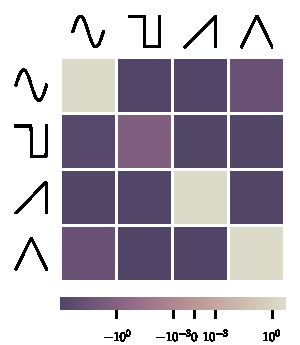
\includegraphics[width=\textwidth]{toy_noise_0/channels_hm.pdf}%
    \caption{0.0}%
    \label{fig:noiseless_channels_toy}%
\end{subfigure}
\begin{subfigure}{0.35\textwidth}
    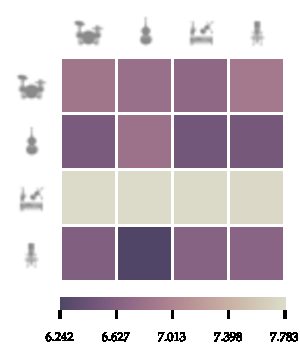
\includegraphics[width=\textwidth]{musdb_noiseless/channels_hm.pdf}%
    \caption{0.0}%
    \label{fig:noiseless_channels_musdb}%
\end{subfigure}

        \end{figure}
        Can we make at least work for the toy data?
    \end{frame}

    \begin{frame}{Noised prior distributions}
        Noiseless distribution is too spiked \(\Rightarrow\) not useable for sampling or variational inference.

        Fine-tune the noiseless models with increasing levels of noised examples to get noised distributions.
    \end{frame}

    \begin{frame}{Experiment: Likelihood of noised inputs}
        \begin{columns}
            \begin{column}{0.5\textwidth}
                How likely are noisy examples under the nosied or noiseless prior distributions?\\
                Here for the \texttt{sine} wave prior.
            \end{column}
            \begin{column}{0.5\textwidth}
                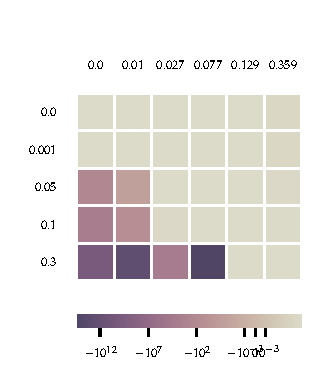
\includegraphics[width=\textwidth]{noised_noised/sin_hm.eps}%
            \end{column}
        \end{columns}
    \end{frame}

    \begin{frame}{Experiment: Cross-likelihood with noised distributions}
        \B{But}, how discriminative are the priors for widening noise-conditioning?
        \begin{figure}
            \centering
            \begin{subfigure}{0.3\textwidth}
                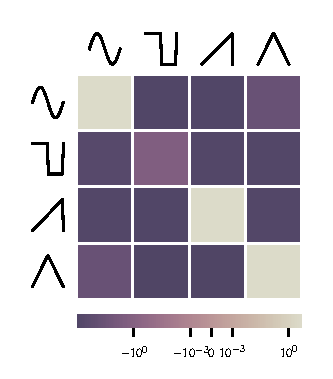
\includegraphics[width=\textwidth]{toy_noise_0/channels_hm.eps}%
                \caption{0.0}%
            \end{subfigure}
            \begin{subfigure}{0.3\textwidth}
                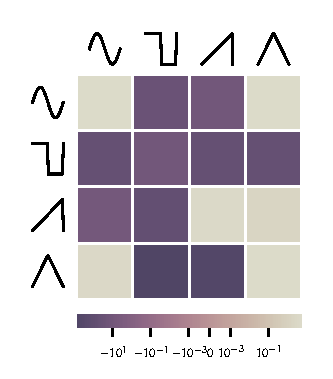
\includegraphics[width=\textwidth]{toy_noise_027/channels_hm.eps}%
                \caption{0.027}
            \end{subfigure}%
            \begin{subfigure}{0.3\textwidth}
                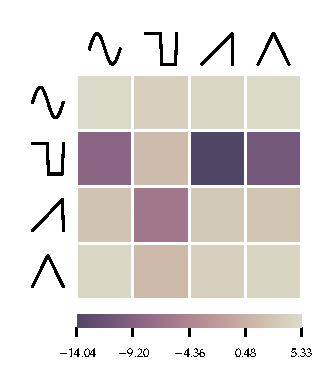
\includegraphics[width=\textwidth]{toy_noise_129/channels_hm.eps}%
                \caption{0.129}
            \end{subfigure}%
        \end{figure}
    \end{frame}

    \begin{frame}{Experiment: Noise and constant inputs}
        Pure noise inputs show destruction of the noisy distribution:
        \begin{figure}
            \centering
            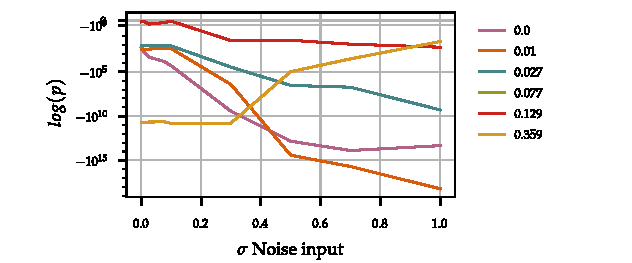
\includegraphics[width=\textwidth]{const_noise_ll.pdf}%
        \end{figure}
    \end{frame}

    \begin{frame}{Experiment: Noise and constant inputs}
        Similar results for constant inputs \(0\) and \(1\):

        \begin{table}
            \begin{tabular}{llrrrr}
\toprule
    &       &      sin &   square &      saw &  triangle \\
value & model &          &          &          &           \\
\midrule
0.0 & 0.0 &  4.8e+00 & -7.0e+02 &  4.4e+00 &   1.8e+00 \\
    & 0.359 & -5.0e-01 & -3.1e+00 &  5.1e+00 &  -2.0e+11 \\
1.0 & 0.0 & -1.5e+01 & -3.6e+03 & -2.7e+06 &  -3.2e+02 \\
    & 0.359 &  2.7e+00 &  4.5e+00 & -2.8e+00 &  -1.1e+01 \\
\bottomrule
\end{tabular}
%
        \end{table}
    \end{frame}

    \begin{frame}{Conclusion}
        \begin{enumerate}
            \item New method for musical source separation without expensive training samples
            \item Fails (so far) because priors are either not discriminative or not smooth enough
            \item Confirm prior work on generative models and out-of-distribution samples
        \end{enumerate}
    \end{frame}

    \begin{frame}[standout]
    \end{frame}
\end{document}
